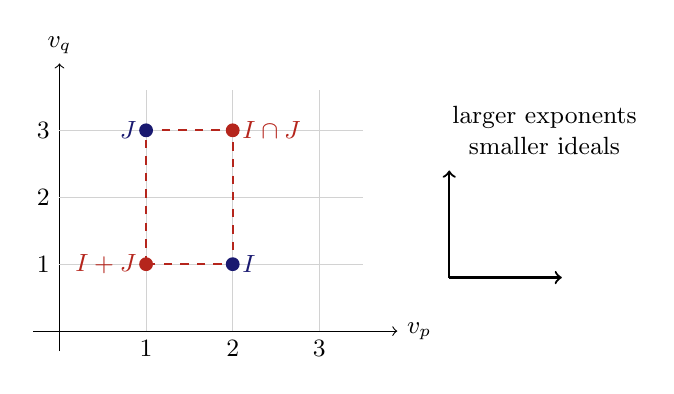
\begin{tikzpicture}[font=\small,x=1.1cm,y=0.85cm]
\draw[->] (-0.3,0)--(3.9,0) node[right] {$v_{\mathfrak p}$};
\draw[->] (0,-0.3)--(0,4.0) node[above] {$v_{\mathfrak q}$};
\foreach \a in {1,2,3} {\draw[gray!35] (\a,0)--(\a,3.6);\node[below] at (\a,0) {$\a$};}
\foreach \b in {1,2,3} {\draw[gray!35] (0,\b)--(3.5,\b);\node[left] at (0,\b) {$\b$};}
\draw[BrickRed,thick,dashed] (1,1) rectangle (2,3);
\fill[MidnightBlue] (2,1) circle (2.5pt) node[right] {$I$};
\fill[MidnightBlue] (1,3) circle (2.5pt) node[left] {$J$};
\fill[BrickRed] (1,1) circle (2.5pt) node[left] {$I+J$};
\fill[BrickRed] (2,3) circle (2.5pt) node[right] {$I\cap J$};
\draw[->,thick] (4.5,0.8)--(5.8,0.8);
\draw[->,thick] (4.5,0.8)--(4.5,2.4);
\node[align=center] at (5.6,3.0) {larger exponents\\smaller ideals};
\end{tikzpicture}
